% !TeX spellcheck = de_DE

\chapter{Installationsanleitung}
\label{chap:install}

\section{Vorbereitende Maßnahmen}
\begin{enumerate}
	\item Splashtop Streamer auf dem ausführenden Laptop installieren
	\item Splashtop Personal auf dem mobilen Anzeigegerät installieren
	\item OpenNI installieren
	\begin{enumerate}
		\item Führen Sie alle \textbf{.MSI} Dateien des OpenNi Ordners aus.
		\item Folgen Sie den Anweisungen der Installationsprozedur.
	\end{enumerate}
	\item PI Connect installieren 
	\begin{enumerate}
		\item Rufen Sie die Datei \textbf{Setup.exe} im zugehörigen PI Connect Ordner auf.
		\item Folgen Sie den Anweisungen der Installationsprozedur.
	\end{enumerate}
	\item Zur erstmaligen Konfiguration PI Conncect starten.
	\item Wählen Sie, wie in \cref{fig:install_config}, unter dem Menüpunkt \textbf{Extras} das Menü \textbf{Konfiguration}
	\begin{figure}[t]
		\centering
		\ifthenelse{\boolean{jpg}}{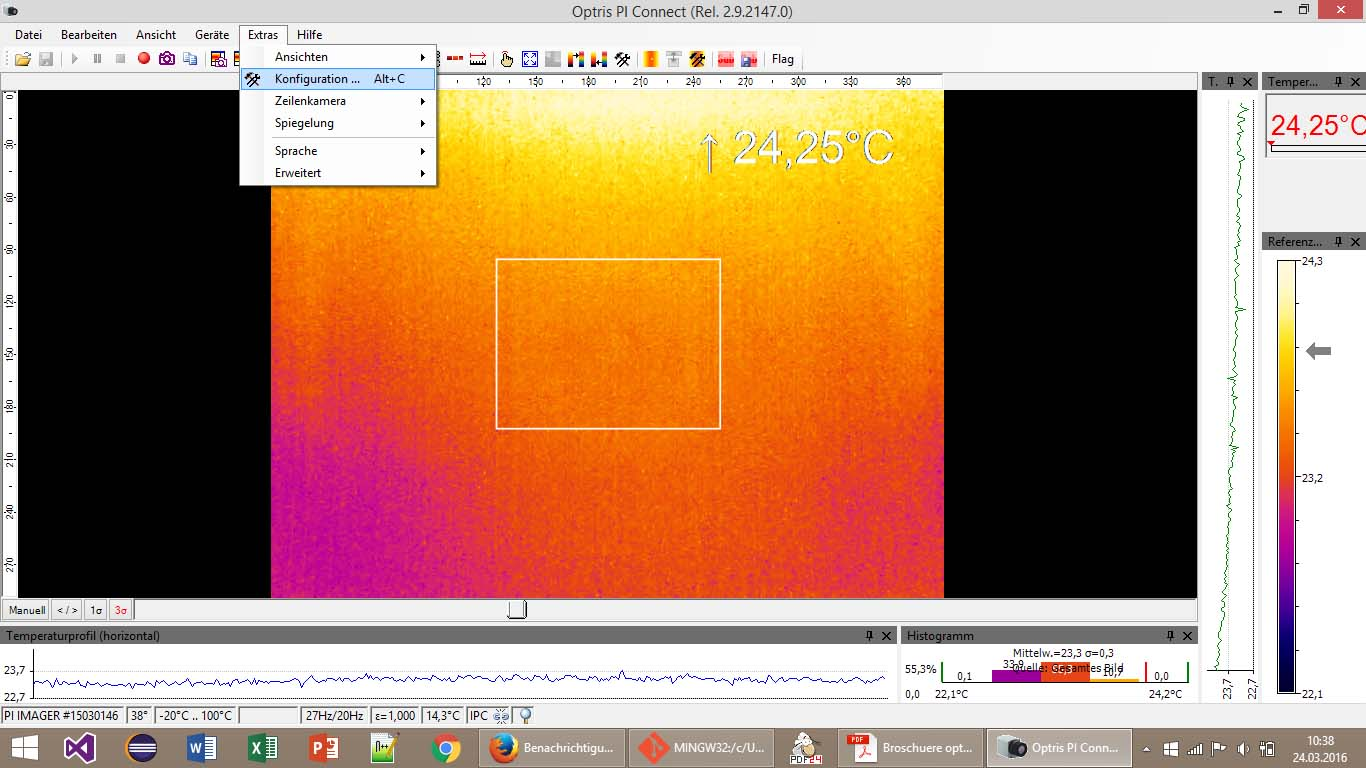
\includegraphics[width=\textwidth]{Install/config.jpg}}{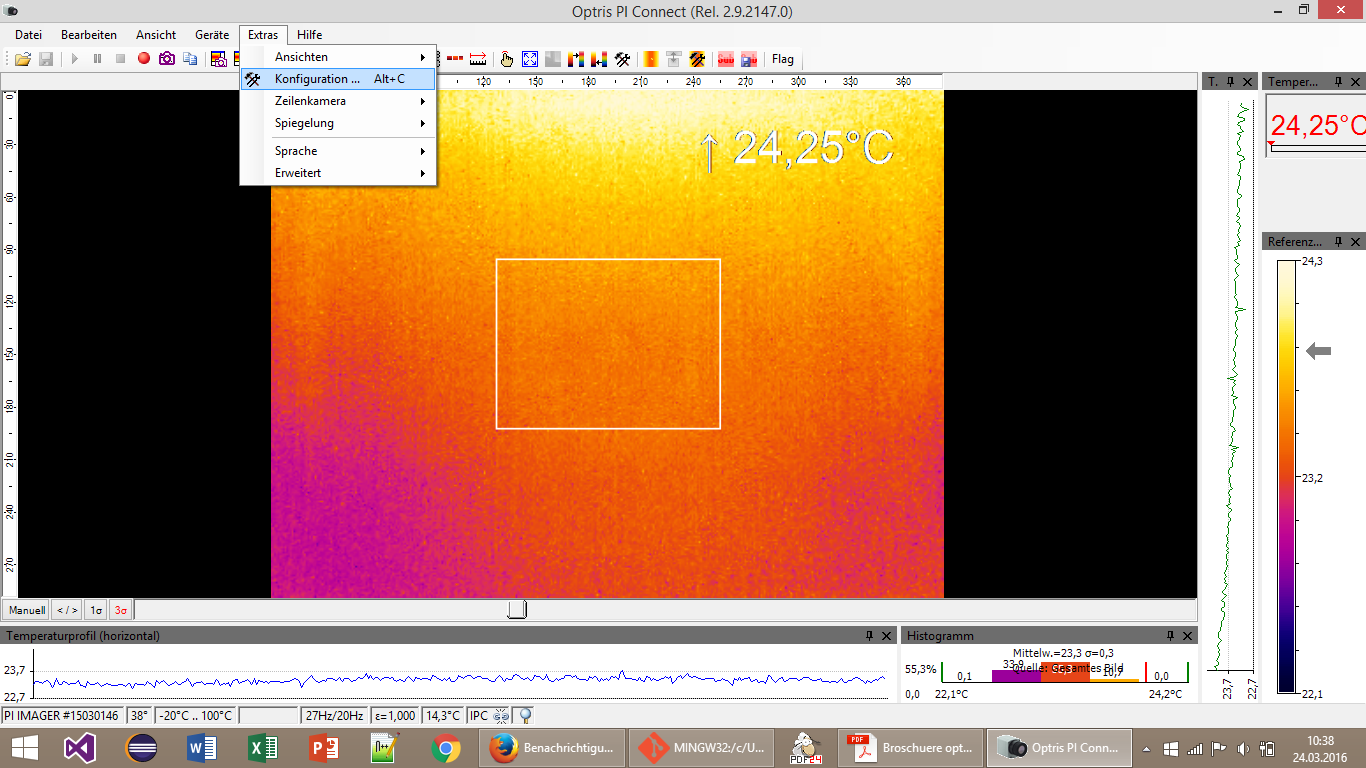
\includegraphics[width=\textwidth]{Install/config.png}}
		\caption{Konfigurationsmenü}
		\label{fig:install_config}
	\end{figure}
	\item Wählen Sie, wie in \cref{fig:install_kommunikation}, den Tab \enquote{\textbf{Externe Kommunikation}} aus und wählen Sie den Modus \textbf{IPC}
	\begin{figure}[t]
		\centering
		\ifthenelse{\boolean{jpg}}{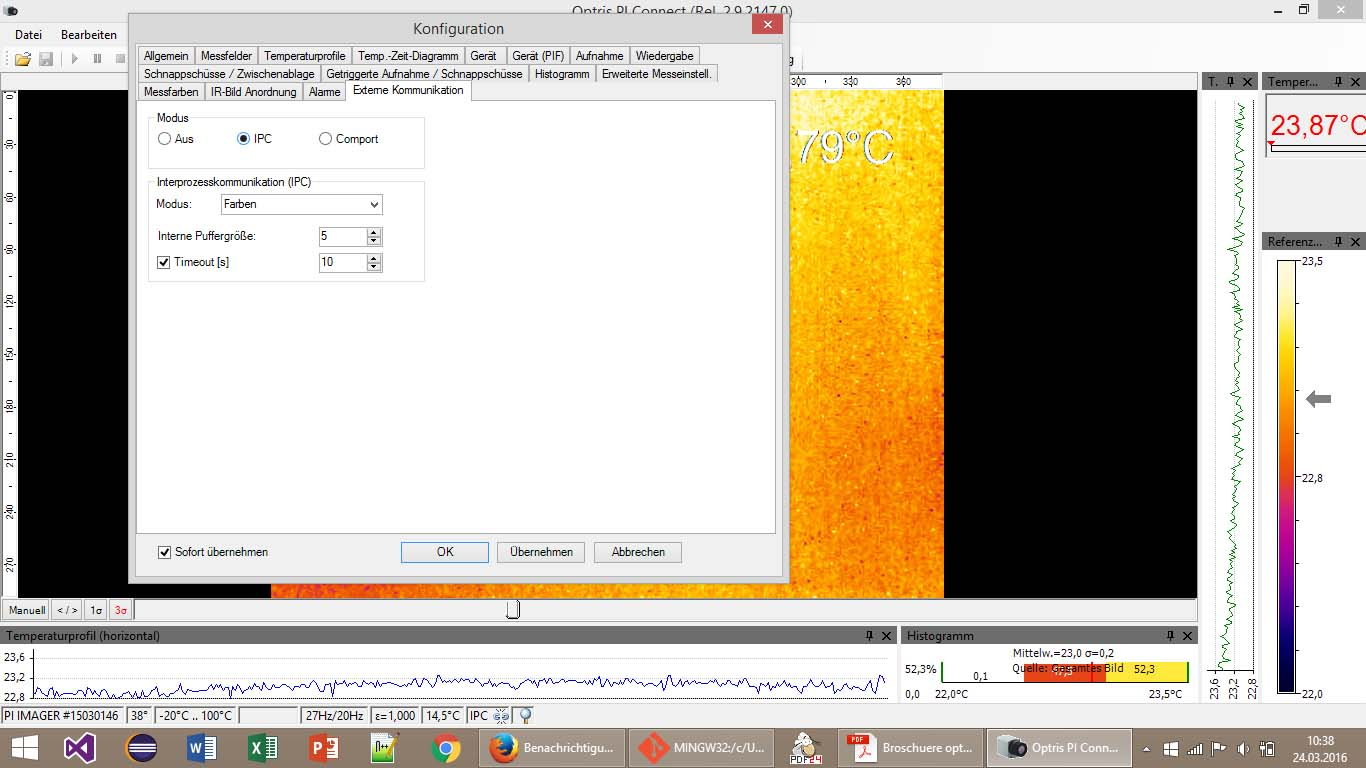
\includegraphics[width=\textwidth]{Install/kommunikation.jpg}}{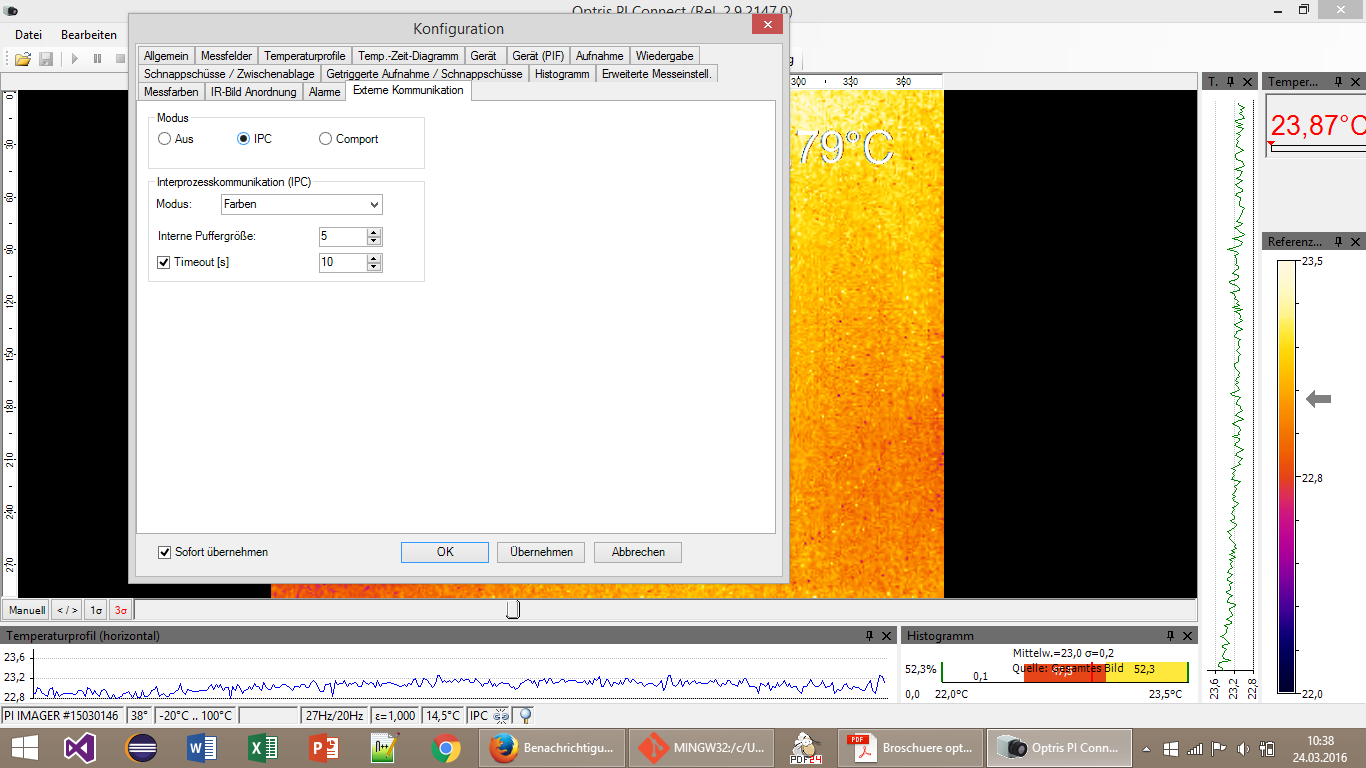
\includegraphics[width=\textwidth]{Install/kommunikation.png}}
		\caption{Einstellungsmenü \textbf{Externe Kommunikation}}
		\label{fig:install_kommunikation}
	\end{figure}
	\item Gehen Sie auf den Tab \enquote{\textbf{Messfelder}}. Führen sie folgende Aktionen durch:
	\begin{enumerate}
		\item Klicken Sie auf die Schaltfläche \enquote{\textbf{Zentrieren}}
		\item Setzen Sie den Wert im Feld \enquote{\textbf{Breite}} (in der \cref{fig:install_messfeld} blau markiert) auf \enquote{\textbf{1}}
		\item Setzen Sie den Wert im Feld \enquote{\textbf{Höhe}} auf \enquote{\textbf{1}}
	\end{enumerate}
	\item Klicken Sie auf nun unten zum Bestätigen auf \textbf{OK}.
	\begin{figure}[H]
		\centering
		\ifthenelse{\boolean{jpg}}{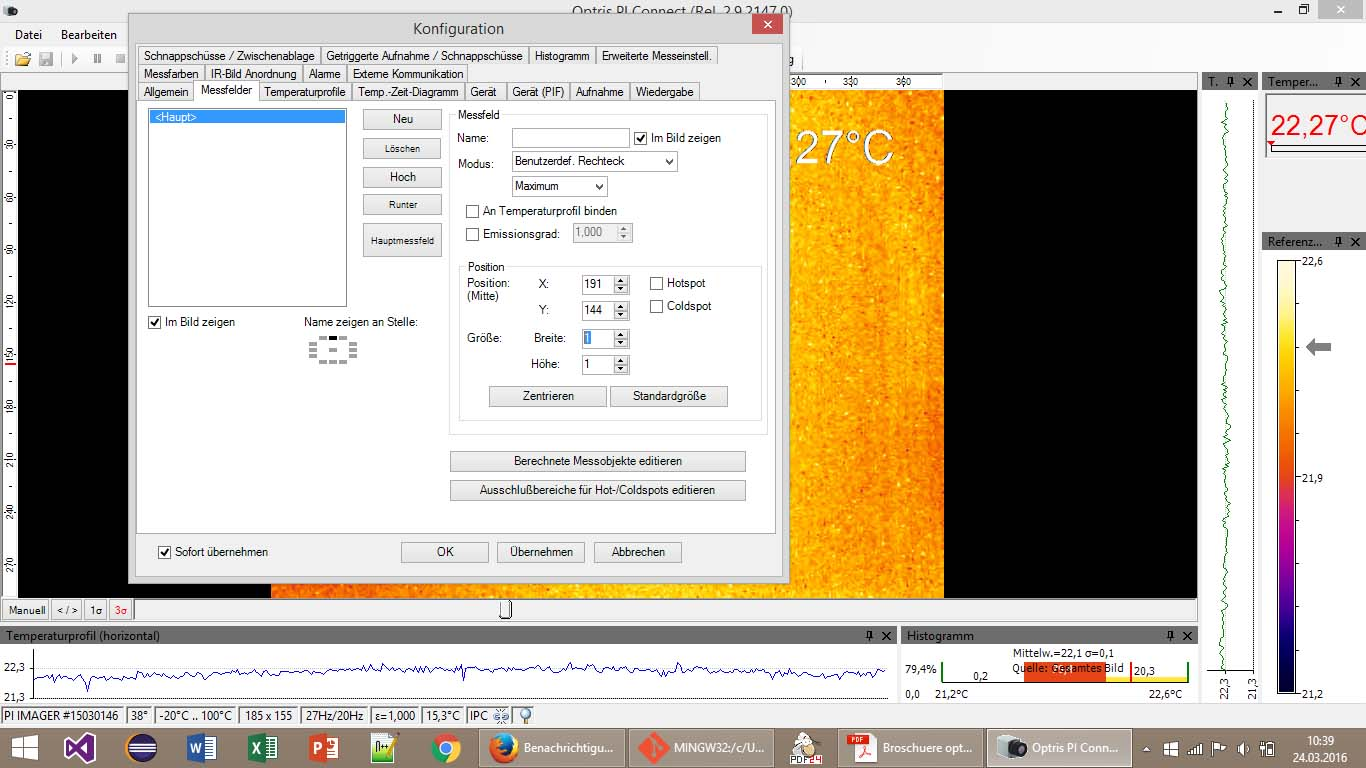
\includegraphics[width=\textwidth]{Install/messfelder.jpg}}{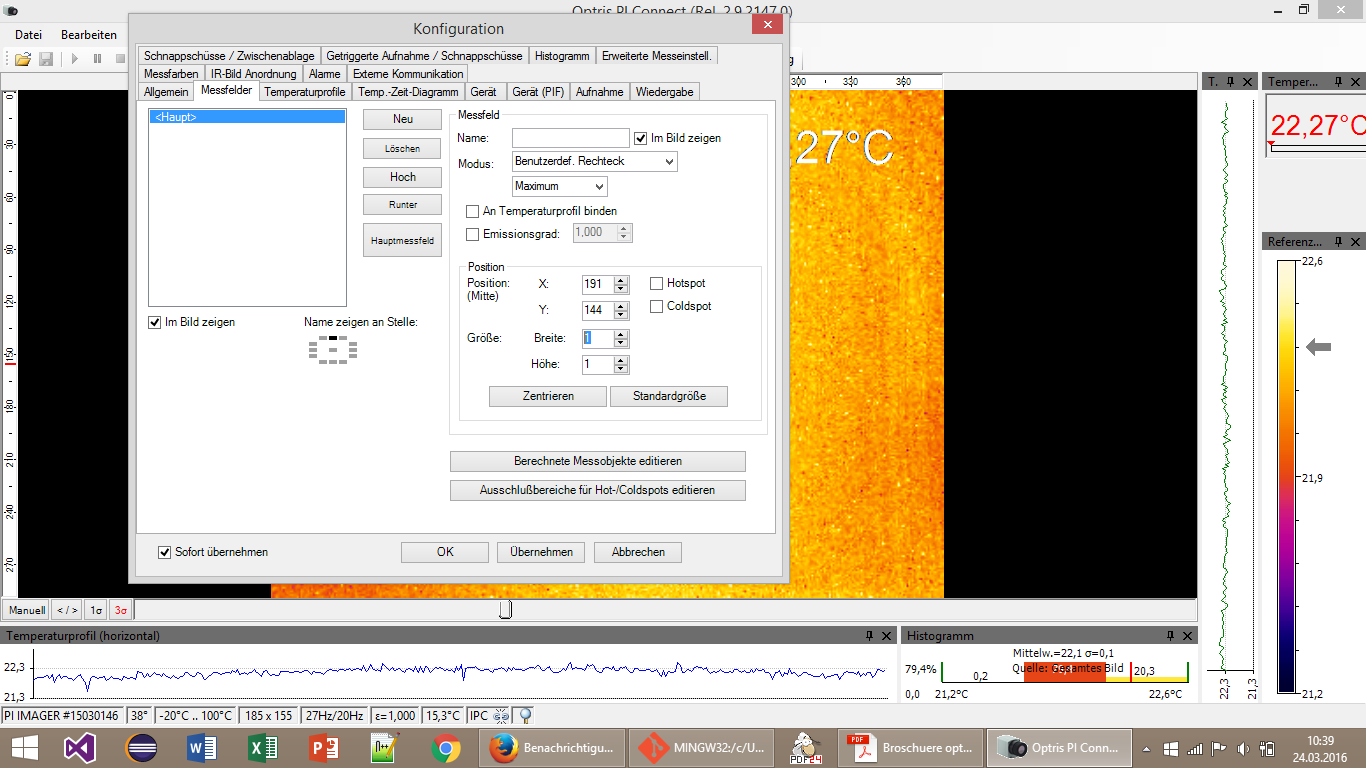
\includegraphics[width=\textwidth]{Install/messfelder.png}}
		\caption{Einstellungsmenü \textbf{Messfelder}}
		\label{fig:install_messfeld}
	\end{figure}
\end{enumerate}

\section{Physischer Aufbau}
\begin{enumerate}
	\item Funkmaus mit dem Laptop verbinden
	\item \meta Anstecken
	\begin{figure}[t]
		\centering
		\begin{subfigure}[t]{0.45\textwidth}
			\centering
			\ifthenelse{\boolean{jpg}}{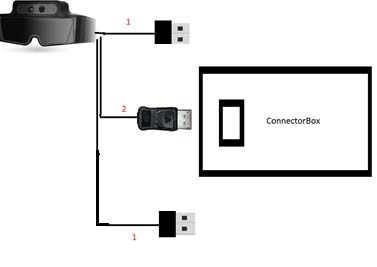
\includegraphics[width=\textwidth]{Install/box.jpg}}{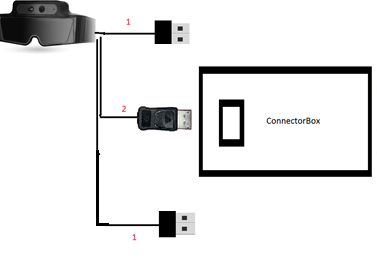
\includegraphics[width=\textwidth]{Install/box.png}}
			\caption{Benötigte Anschlüsse der \meta}
			\label{fig:install_box}
		\end{subfigure}
		~
		\begin{subfigure}[t]{0.45\textwidth}
			\centering
			\ifthenelse{\boolean{jpg}}{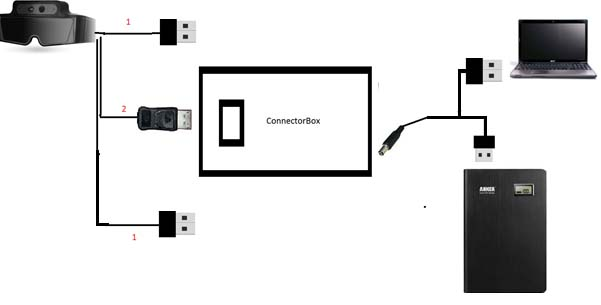
\includegraphics[width=\textwidth]{Install/akku.jpg}}{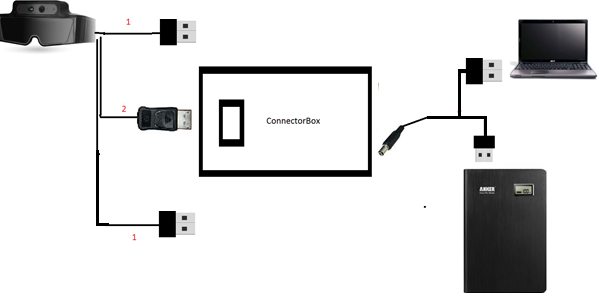
\includegraphics[width=\textwidth]{Install/akku.png}}
			\caption{Benötigte Anschlüsse des Akkus}
			\label{fig:install_akku}
		\end{subfigure}
		\caption{Andeutung der benötigten Anschlüsse}
		\label{fig:install_power}
	\end{figure}
	\begin{figure}[t]
		\centering
		\begin{subfigure}[t]{0.45\textwidth}
			\centering
			\ifthenelse{\boolean{jpg}}{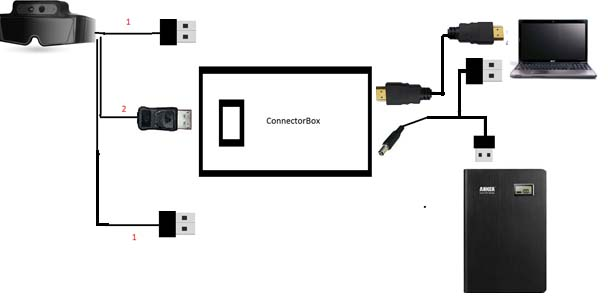
\includegraphics[width=\textwidth]{Install/hdmi.jpg}}{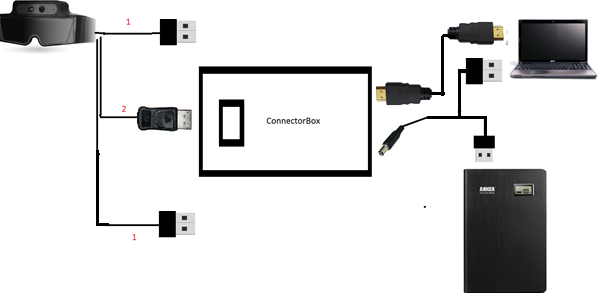
\includegraphics[width=\textwidth]{Install/hdmi.png}}
			\caption{HDMI Verbindung der \meta über die Controllerbox an den Laptop}
			\label{fig:install_hdmi}
		\end{subfigure}
		~
		\begin{subfigure}[t]{0.45\textwidth}
			\centering
			\ifthenelse{\boolean{jpg}}{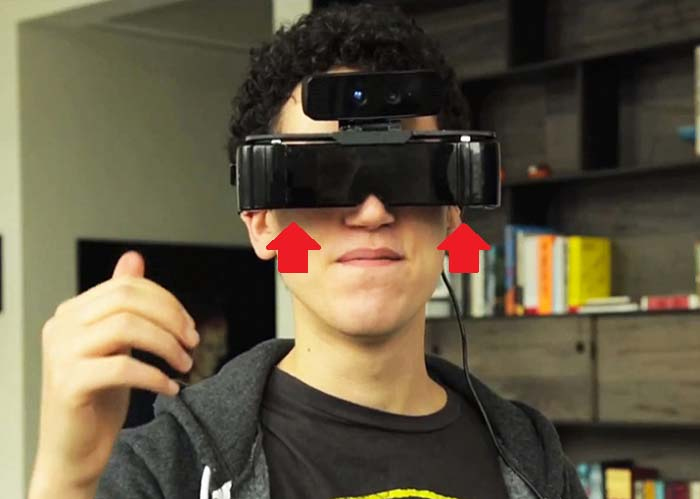
\includegraphics[width=\textwidth]{Install/meta.jpg}}{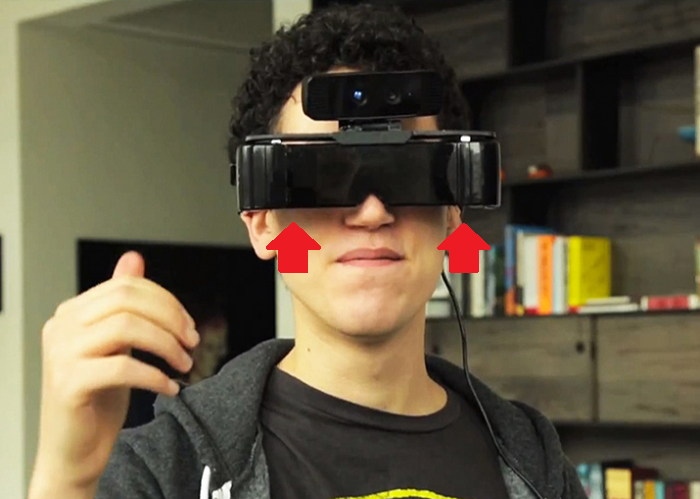
\includegraphics[width=\textwidth]{Install/meta.png}}
			\caption{Getragene \meta}
			\label{fig:install_meta}
		\end{subfigure}
		\caption{Abgeschlossenes \setup}
		\label{fig:install_setup}
	\end{figure}
	\begin{enumerate}
		\item Das Bildübertragungskabel (2) der \meta Brille, wie in \cref{fig:install_box} angedeutet, in die dazugehörige Connector Box einstecken und beide USB-Ports der \meta nicht verbinden.
		\item Im nächsten Schritt wird das Y-USB-Stromkabel mit der runden Seite in die Connectorbox gesteckt.
		Von beiden anderen Enden, welche aus jeweils einem USB-Stecker bestehen wird anschließend ein Ende in den Akku gesteckt und das andere gelangt in den dazugehörigen Laptop. Dies ist in \cref{fig:install_akku} angedeutet.
		\item Im dritten Schritt wird, wie in \cref{fig:install_hdmi} angedeutet, das HDMI-Kabel an die ConnectorBox und den Laptop angesteckt.
		\item Akku anschalten und warten bis die Brille startet dann ist die Brille einsatzbereit.
		\item Nun kann man dann die Brille aufsetzen und Linsen der Brille unten an der Brille ausrichten. Diese Stellen sind in \cref{fig:install_meta} markiert.
	\end{enumerate}
	\item Falls die \textit{Helmhalterung} genutzt werden soll: Halterung an de vorgesehenen Stelle anbringen und Helm aufsetzen.
	
	Falls die \textit{Handhalterung} genutzt werden soll: Handy in der dafür vorgesehenen Halterungskerbe platzieren.
\end{enumerate}

\section{Programmstart}
\begin{enumerate}
	\item Splashtop Streamer auf dem Laptop starten
	
	Vorhandenes Benutzerkonto
	\begin{description}
		\item[User] abc12g3@trash-mail.com
		\item[Passwort] 123456
	\end{description}
	\item PI Connect starten und warten bis der Startvorgang vollendet ist
	\item \textbf{start\_network.bat} ausführen
	\item \textbf{ProFire\_v.1.0.exe} ausführen
	\item Splashtop Personal auf dem Handy starten
	\item Mit lokalem Netzwerk verbinden
	\begin{description}
		\item[SSID] profire
		\item[Passwort] 12345678
	\end{description}
\end{enumerate}